%% ExoColumn manuscript
%% AASTeX v7.0.1 -- target journal: ApJ
%%
%% Style options (see aastex701 documentation for the full list):
%%   twocolumn / manuscript / preprint / preprint2 / modern -- typesetting styles
%%   linenumbers  -- line numbering (mandatory for AAS submission)
%%   trackchanges -- show \added/\replaced/\deleted markup
%%
\documentclass[linenumbers]{aastex701}

%% Figures are referenced in place from the repository's reference/ tree
%% (no copies are kept in ms/). Paths below are written relative to the repo
%% root; the two graphicspath entries make this resolve whether the LaTeX
%% compiler runs from ms/ (../) or from the project root (./).
\graphicspath{{../}{./}}

%% Running heads (shown on alternating pages).
\shorttitle{ExoColumn}
\shortauthors{Haqq-Misra}

%% Target journal.
\submitjournal{ApJ}

\begin{document}

%% ============================================================
%% Front matter
%% ============================================================

\title{Placeholder Title: A One-Dimensional Radiative--Convective Model for Exoplanet Habitable-Zone Studies}

\author{Jacob Haqq-Misra}
\affiliation{Blue Marble Space Institute of Science, Seattle, WA, USA}
\email[show]{jacob@bmsis.org}

%% [Co-authors added per request. Affiliations are my best guess -- please
%% verify/replace, and add ORCIDs and \email{} addresses as appropriate.]
\author{Eric T. Wolf}
\affiliation{[Laboratory for Atmospheric and Space Physics, University of Colorado Boulder, Boulder, CO, USA]}

\author{Ravi Kopparapu}
\affiliation{[NASA Goddard Space Flight Center, Greenbelt, MD, USA]}

%% Additional authors go here.

\begin{abstract}
%% TODO: abstract (250-word limit for ApJ).
\end{abstract}

%% TODO: select UAT keywords -- https://astrothesaurus.org
%% [Suggested UAT concepts (grab the numeric IDs from astrothesaurus.org):
%% Habitable zone; Exoplanet atmospheres; Planetary atmospheres; Radiative
%% transfer; Extrasolar rocky planets; Planetary climates.]
\keywords{}

%% ============================================================
%% Body
%% ============================================================

\section{Introduction} \label{sec:intro}
%% TODO
[One-dimensional radiative--convective equilibrium (RCE) models are the standard
tool for computing habitable-zone (HZ) limits (Kasting et al. 1993; Kopparapu
et al. 2013, 2014). ExoColumn pairs a conventional RCE column with the ExoRT
correlated-$k$ radiation package used by the ExoCAM GCM, so its 1-D radiation is
consistent with 3-D simulations. This paper documents the model and validates it
against (i) modern Earth, (ii) line-by-line (LBL) radiative-transfer benchmarks,
and (iii) the Kopparapu et al. (2013, 2014) HZ limits, then provides updated HZ
boundary coefficients (Table~\ref{tab:hz_coeff}) for community use.]

\section{The ExoColumn model} \label{sec:model}
%% TODO
[ExoColumn is a 1-D RCE model that calls ExoRT's \texttt{aerad\_driver}
radiation routine directly (the same correlated-$k$ core as ExoCAM), using the
n68equiv 68-band scheme. Vertical grid: default 70 layers, log-spaced from
$p_{\rm top}$ to the surface; layer count is a compile-time constant. Convection
(default): simplified Betts--Miller (SBM; Frierson 2007), relaxing temperature to
the moist adiabat and humidity to a reference RH (0.7); four other schemes are
selectable. Surface turbulent fluxes: simplified Monin--Obukhov (Frierson 2006)
with the drag coefficient referenced at a fixed 10 m height (resolution-
independent, $C\approx10^{-3}$), paired with a surface-coupled mixed layer --- no
separate boundary-layer scheme. Water vapour is prognostic, with a cold-point
(Brewer--Dobson) stratospheric cold trap. The surface is a slab ocean
($H_{\rm slab}=4.1\times10^{7}\,{\rm J\,m^{-2}\,K^{-1}}$ for a 10 m layer) evolved
with semi-implicit Planck damping. Adaptive CFL timestep $\in[10^{-4},1]$ day
with $\Delta T_{\rm target}=1$ K. Optional physics, all default-off (results
bit-identical when off): IAPWS-95 non-ideal steam EOS (Wagner \& Pru\ss\ 2002)
with the Kasting (1988) non-ideal moist adiabat; the BPS/Wolf H$_2$O continuum;
and CO$_2$ condensation with $T$-dependent $c_p$ for the outer HZ. The model is
Fortran; ExoRT is used unmodified.]

\section{Earth validation} \label{sec:earth}
%% TODO
[Modern-Earth cold start (1 bar N$_2$/O$_2$/Ar, 400 ppm CO$_2$, RCEMIP O$_3$),
surface albedo calibrated to $T_s=288$ K. The equilibrium is insensitive to the
convective closure: holding all else fixed and swapping SBM for the fixed
6.5 K km$^{-1}$ (Manabe) and RH-weighted moist-adiabat schemes shifts $T_s$ by
only $+1.5$ and $+2.2$ K (the Zhang--McFarlane soft scheme runs $+7.5$ K warmer).
The cold-point minimum ($\approx$204 K) is $\sim$7 K warmer than konrad's RRTMG
($\approx$197 K), attributable to ExoRT-n68equiv vs RRTMG radiation differences.]

\begin{figure}[ht!]
\centering
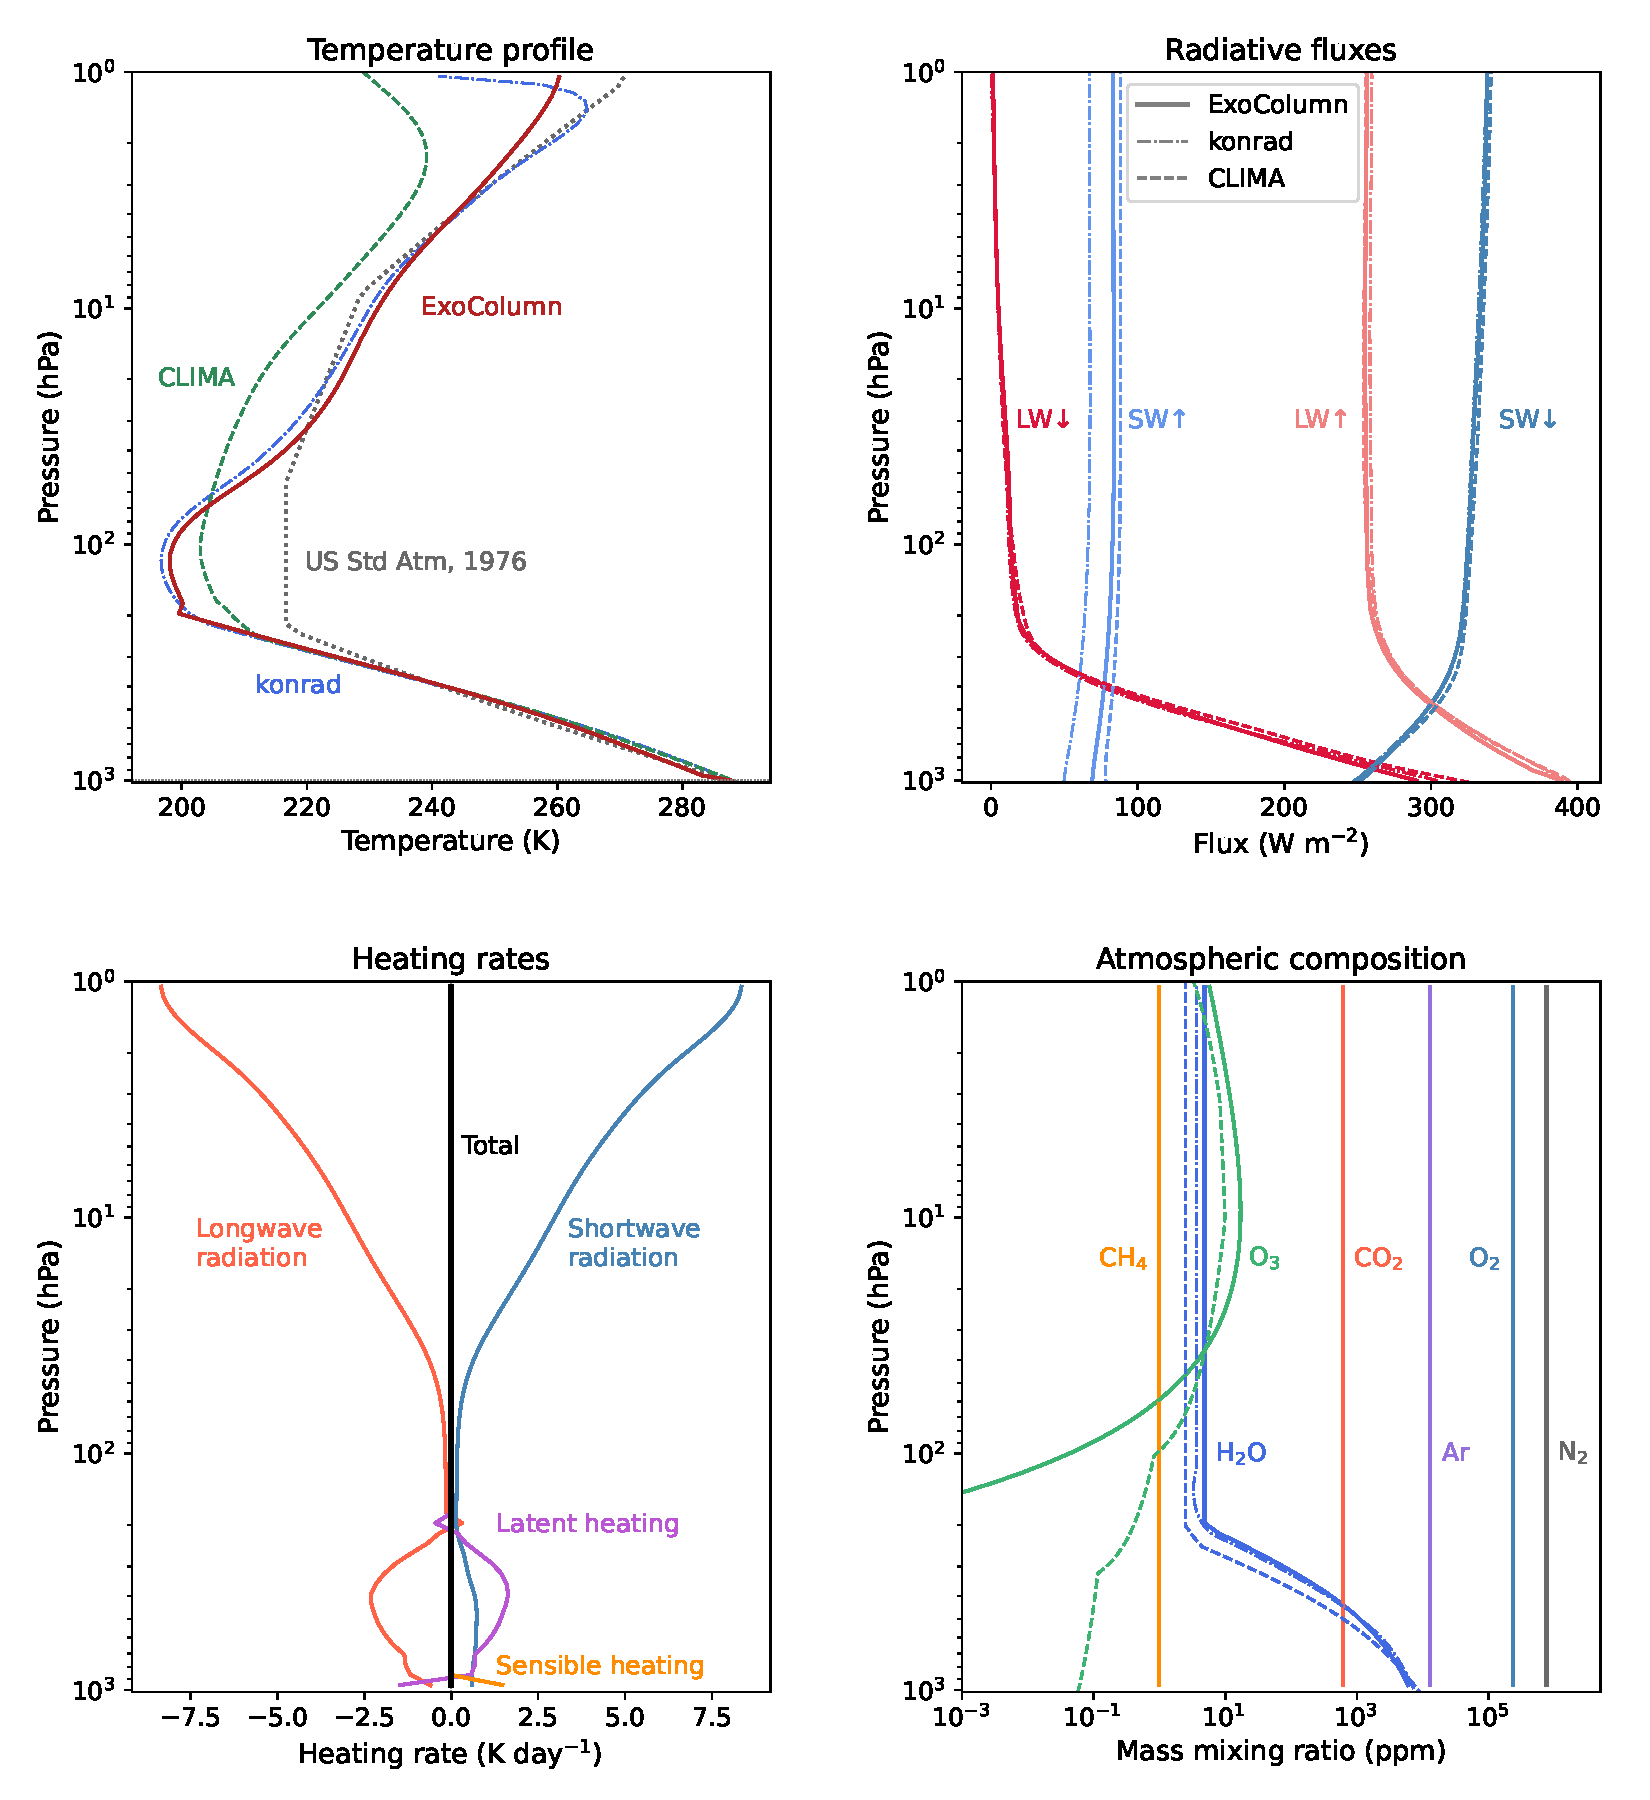
\includegraphics[width=0.8\textwidth]{reference/earth/earth_rce.pdf}
\caption{[Modern-Earth RCE. Panels: (a) temperature profile, (b) radiative
fluxes, (c) heating rates, (d) water vapour. ExoColumn (surface albedo 0.2736)
gives $T_s=287.84$ K, cold-point minimum $\approx204$ K, latent/sensible heat
fluxes 68.0/16.4 W m$^{-2}$ (Bowen ratio 0.24), and precipitation
2.35 mm day$^{-1}$; converged in 2107 steps ($\approx$1000 model days) to a TOA
imbalance $<0.1$ W m$^{-2}$. Compared with konrad (RRTMG), CLIMA, and the US
Standard Atmosphere 1976 (dotted).]}
\label{fig:earth_rce}
\end{figure}

\section{Radiative-transfer benchmarks} \label{sec:lbl}
%% TODO
[Independent LBL check of the ExoRT n68equiv core (built with a
numba Lorentz$\times\chi$ code: Perrin--Hartmann 1989 $\chi$-factor plus
HITRAN-2024 CO$_2$--CO$_2$ CIA). The dense-CO$_2$ window OLR is governed by the
CO$_2$ far-wing/$\chi$ treatment and spans a wide envelope; ExoRT lands inside
it, near CLIMA. Both correlated-$k$ cores are LBL-grade (F$_{\rm IR}$ within 1\%,
SW albedo within 0.0002 of LBL), so the model-to-Kopparapu offsets quantified
later are CLIMA-2013 ingredient differences, not radiation-core errors.]

\begin{figure*}[ht!]
\centering
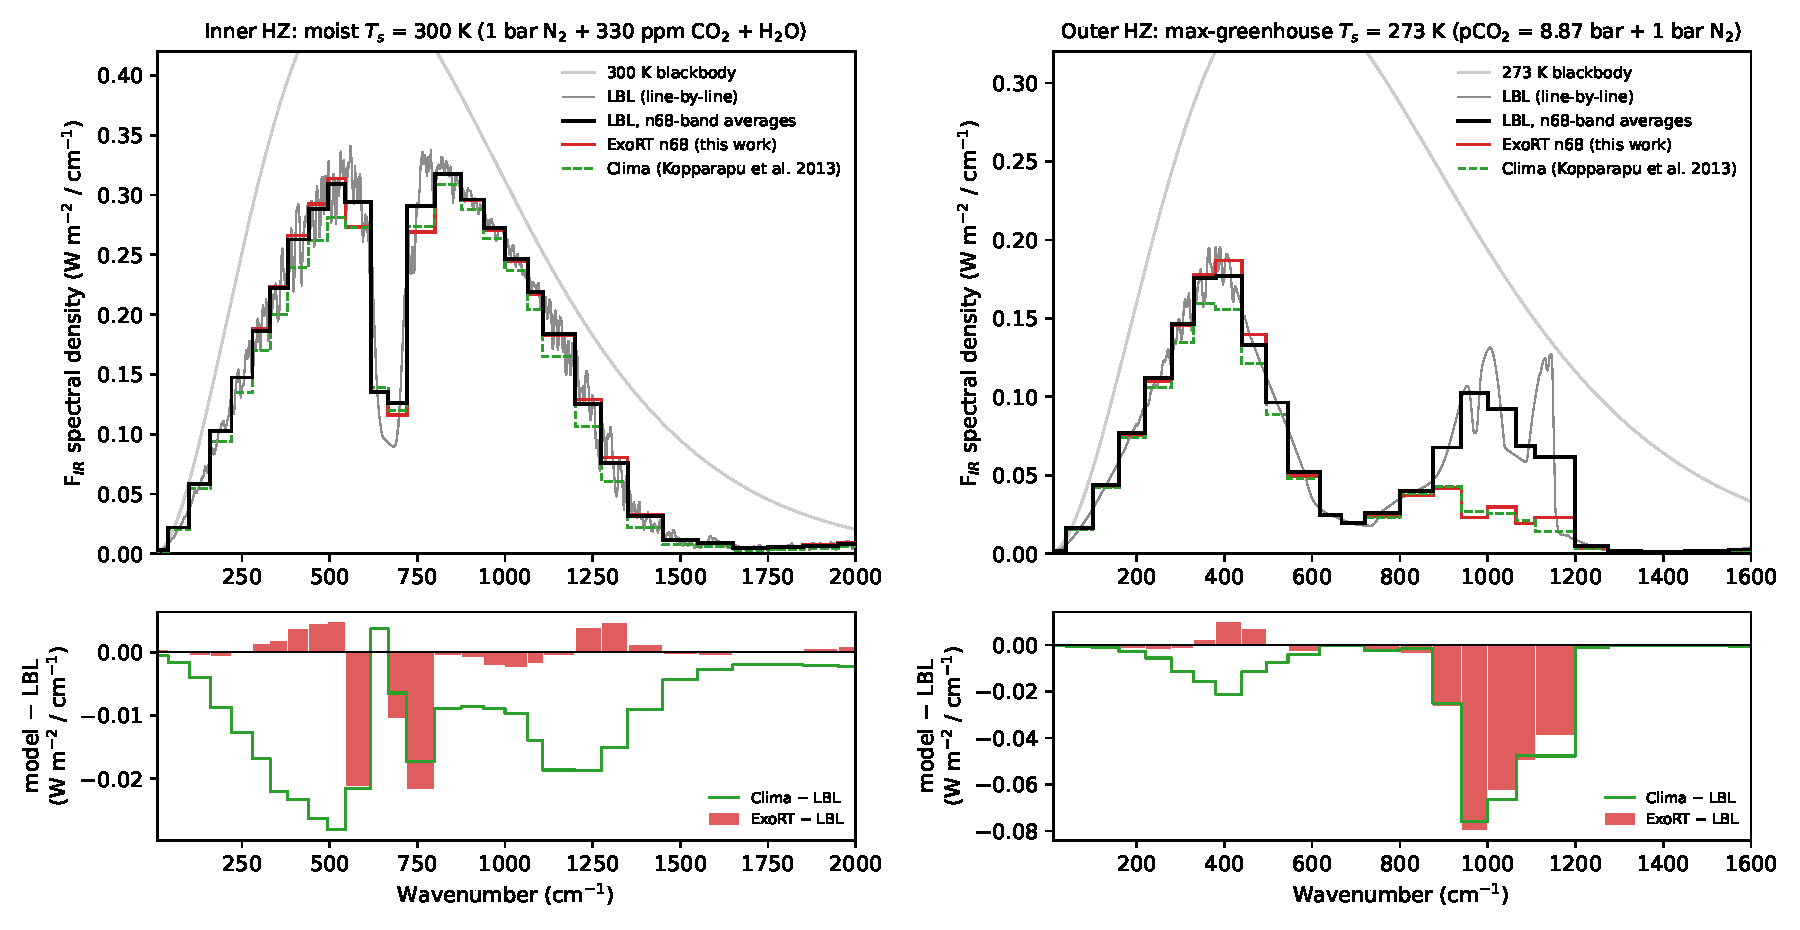
\includegraphics[width=\textwidth]{reference/max_greenhouse/lbl_olr_benchmark_2panel.pdf}
\caption{[LBL validation of the ExoRT n68equiv core. Left: inner-HZ-like column
($T_s=300$ K). Right: outer-HZ dense-CO$_2$ column (8.87 bar). Grey = LBL
reference, black = n68 band averages, red = ExoRT, green = CLIMA (2013-era and
Wolf 2016). For the dense-CO$_2$ window the OLR ranges from $\approx$44 (pure
Lorentz) to $\approx$92 W m$^{-2}$ (PH89 $\chi$); ExoRT (75.5) and CLIMA
(69--72) both sit inside this envelope. The window spread is set by the CO$_2$
far wings, not by CIA (negligible there in both HITRAN and ExoRT).]}
\label{fig:lbl}
\end{figure*}

\section{The inner edge of the habitable zone} \label{sec:inner}
%% TODO
[Inner-edge sweep for a Sun-like star using the non-ideal (IAPWS-95) steam EOS;
the figure compares the default MT\_CKD continuum, the BPS continuum, and CLIMA.
OLR asymptotes to the Simpson--Nakajima limit $\approx$295 W m$^{-2}$ (Kopparapu
291; 1.3\% high). With MT\_CKD: moist-greenhouse limit $S_{\rm eff}=1.087$
($d=0.959$ AU) and runaway-greenhouse limit $S_{\rm eff}=1.101$ ($d=0.953$ AU);
the BPS continuum lowers these to 1.074/1.093 and CLIMA gives 1.016/1.060. The
residual $S_{\rm eff}$ offset vs CLIMA is near-IR shortwave H$_2$O absorption
(our albedo plateau 0.211 vs CLIMA's 0.193), consistent with the LBL
decomposition in Section~\ref{sec:lbl}; the OLR itself matches to 1.3\%.]

\begin{figure*}[ht!]
\centering
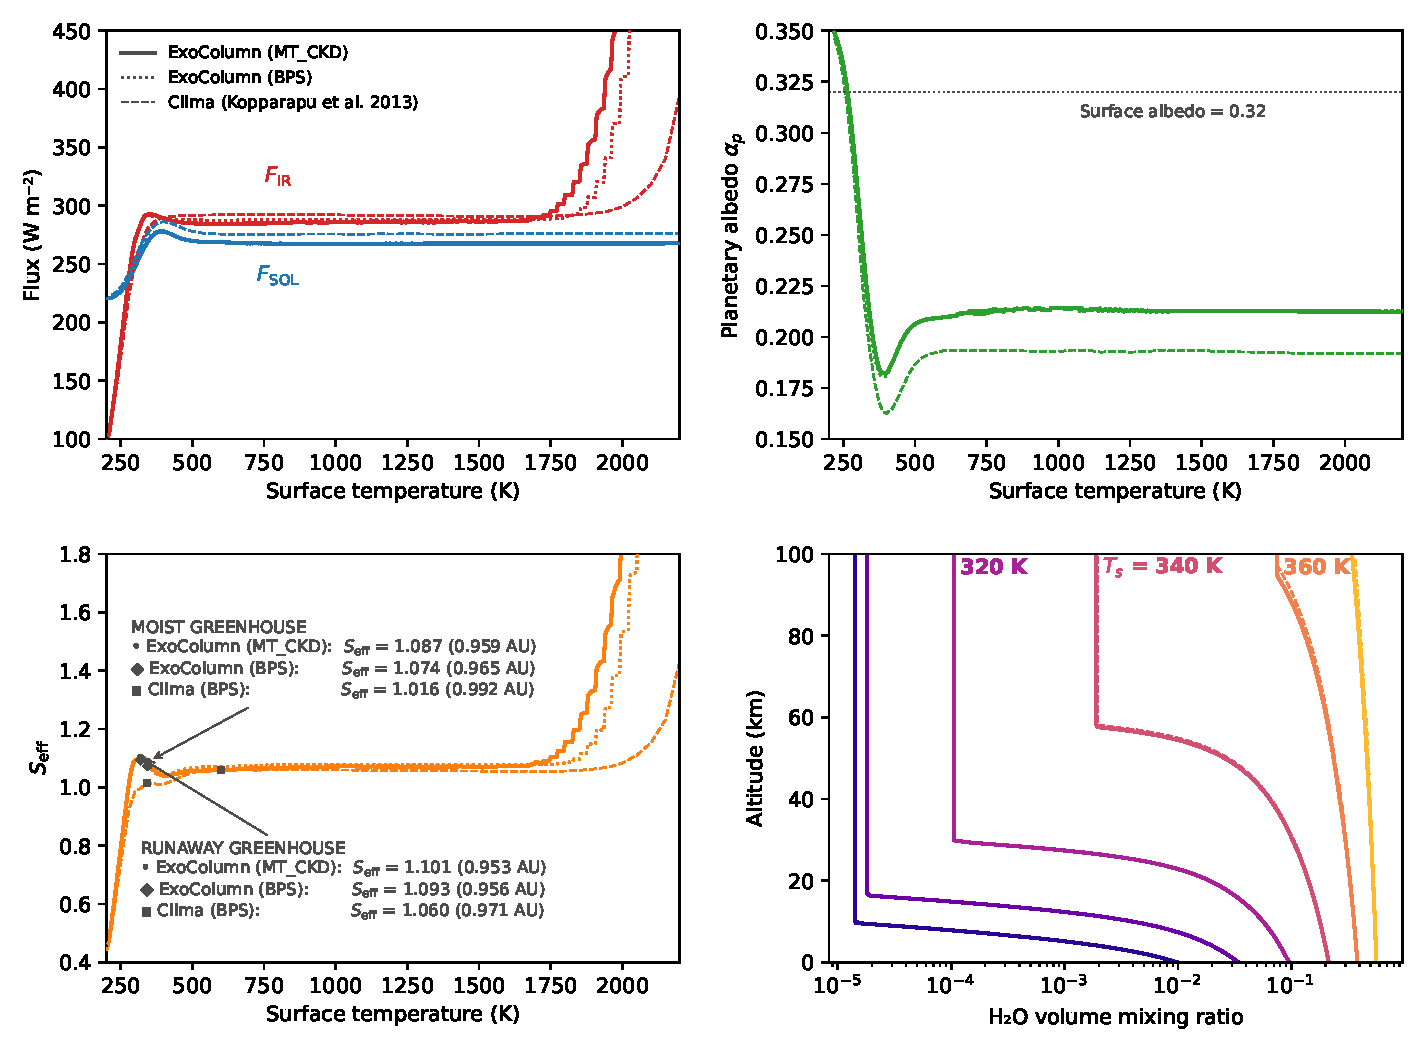
\includegraphics[width=\textwidth]{reference/moist_runaway/hz_inner_nonideal.pdf}
\caption{[Inner edge of the HZ for a Sun-like star (analogue of Kopparapu et al.
2013, Fig. 3). Panels (a)--(c): OLR, planetary albedo, and effective stellar
flux $S_{\rm eff}$ vs surface temperature for the MT\_CKD (default) and BPS
continua and CLIMA; panel (d): H$_2$O volume mixing ratio profiles (altitude vs
VMR) at $T_s$ = 320, 340, 360 K. OLR caps near the Simpson--Nakajima limit
($\approx$295 W m$^{-2}$); the moist-greenhouse ($S_{\rm eff}=1.087$, 0.959 AU)
and runaway-greenhouse ($S_{\rm eff}=1.101$, 0.953 AU) limits are marked
(MT\_CKD). Dashed/markers = Kopparapu/CLIMA (2013) data.]}
\label{fig:hz_inner}
\end{figure*}

\section{The outer edge of the habitable zone} \label{sec:outer}
%% TODO
[Maximum-greenhouse (outer-edge) CO$_2$ sweep, 1--34.7 bar, for a Sun-like star,
with CO$_2$ condensation and $T$-dependent $c_p$ enabled. Maximum greenhouse at
$S_{\rm eff}=0.395$ ($p_{\rm CO_2}=8.9$ bar, $d=1.59$ AU) vs Kopparapu 0.343
($\approx$7 bar, 1.70 AU); ours is the more conservative (closer-in) outer bound,
pushed high by the dense-CO$_2$ radiation offset (albedo converges onto
Kopparapu's by 35 bar). Caveat: above 10 bar the $k$-coefficient pressure lookup
is clamped at the table top (ExoRT extrapolates beyond its grid), freezing
pressure broadening at its 10 bar value while CIA/continuum use the true
pressure.]

\begin{figure}[ht!]
\centering
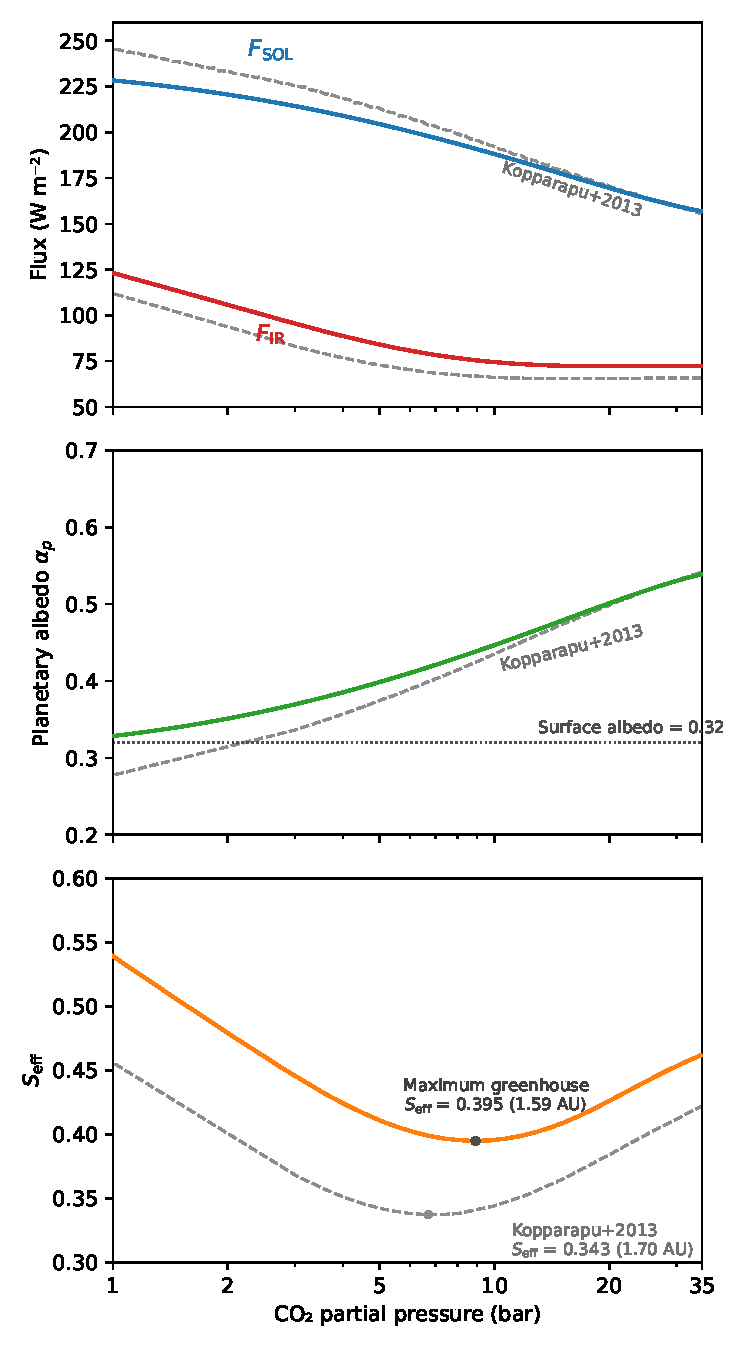
\includegraphics[width=0.45\textwidth]{reference/max_greenhouse/hz_outer.pdf}
\caption{[Outer edge of the HZ for a Sun-like star (analogue of Kopparapu et al.
2013, Fig. 5): effective stellar flux $S_{\rm eff}$ vs CO$_2$ partial pressure
over a 1--34.7 bar sweep. The maximum-greenhouse limit (minimum $S_{\rm eff}$)
is $0.395$ at 8.9 bar ($d=1.59$ AU); Kopparapu's is 0.343 at $\approx$7 bar.
Dashed/markers = Kopparapu (2013).]}
\label{fig:hz_outer}
\end{figure}

\section{Habitable-zone limits across stellar spectral types} \label{sec:stellar}
%% TODO
[HZ limits computed for nine host stars spanning F (7200 K) through G (5780 K,
Sun), K (4000--4800 K), and M (2600--3700 K), using BT-Settl SEDs (the cool-star
set is extended down to 2000 K). The host SED enters the cold-start column only
through albedo, so the moist-greenhouse limit falls at a star-independent
$T_s=344$ K and only $S_{\rm eff}$ differs between stars. The fitted boundary
coefficients (Table~\ref{tab:hz_coeff}) reproduce the Kopparapu quartic form
$S_{\rm eff}=S_{\rm eff,\odot}+a\,T_\star+b\,T_\star^2+c\,T_\star^3+d\,T_\star^4$
($T_\star=T_{\rm eff}-5780$ K) and fit the model results to RMS $\sim10^{-3}\,
S_\odot$ over 2000--7200 K; they are a drop-in replacement for Kopparapu's
Table 3 with the ExoColumn radiation core ($S_{\rm eff,\odot}=1.10$, 1.09, and
0.39 for the runaway-, moist-, and maximum-greenhouse limits).]

\begin{figure*}[ht!]
\centering
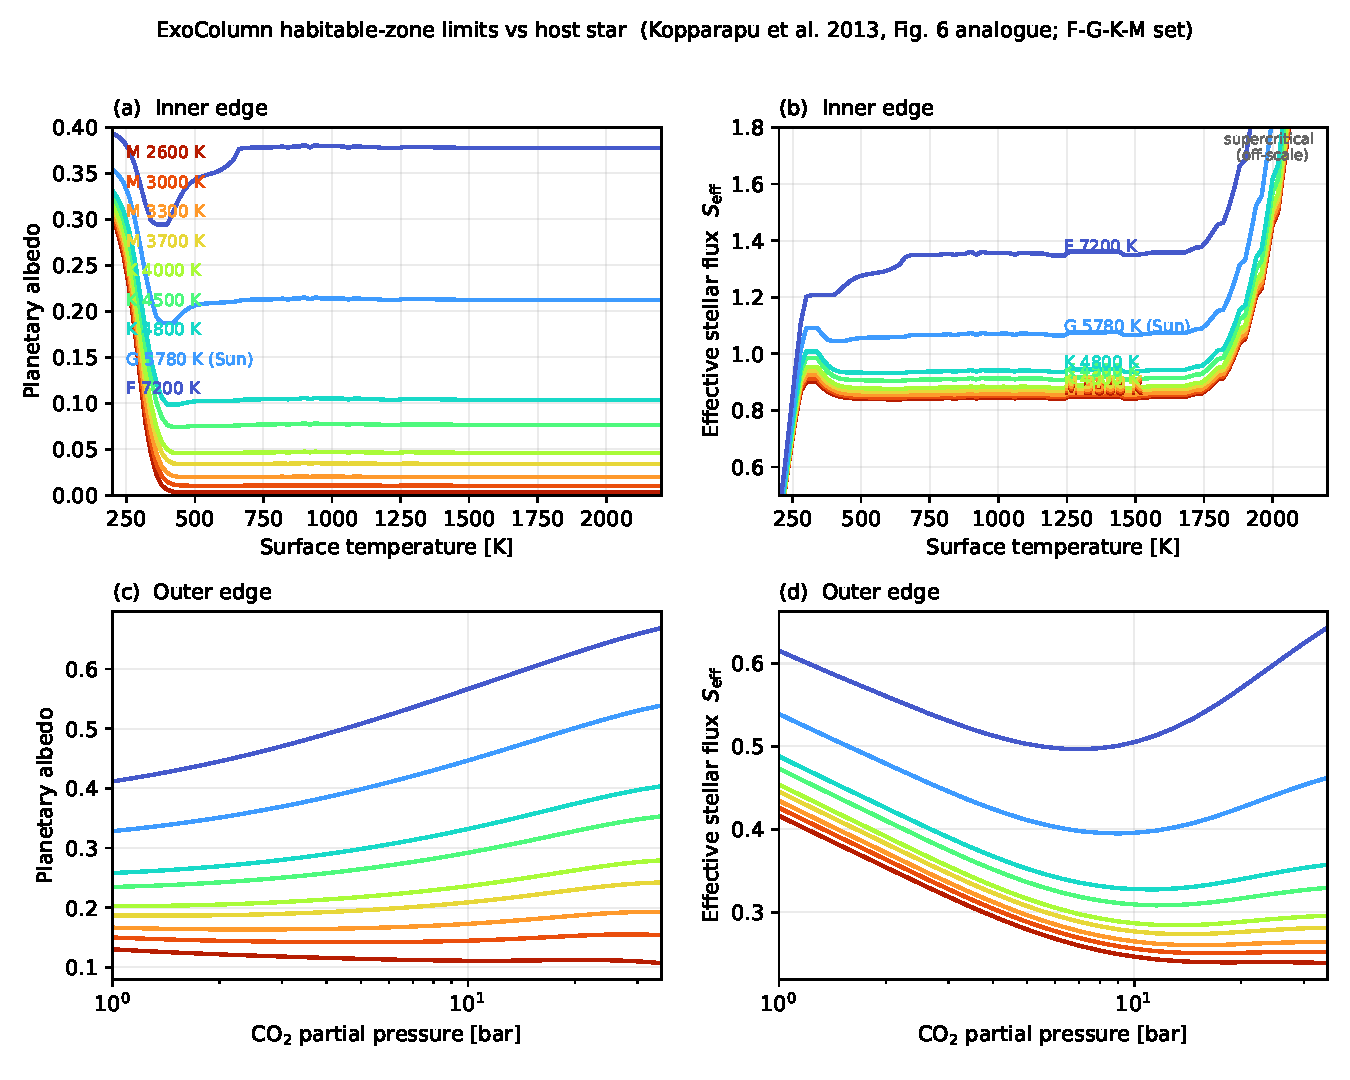
\includegraphics[width=0.95\textwidth]{reference/habitablezone/hz_figure6.pdf}
\caption{[HZ limits across stellar type (analogue of Kopparapu et al. 2013,
Fig. 6): planetary albedo and effective stellar flux $S_{\rm eff}$ vs (top)
surface temperature and (bottom) CO$_2$ partial pressure, for nine host stars
from M (2600 K) to F (7200 K). Maximum-greenhouse $S_{\rm eff}$ rises from 0.239
(M, 2600 K) through 0.395 (G, Sun) to 0.497 (F, 7200 K): cooler, redder stars
have lower albedo (more near-IR absorption), warming the column and shifting the
HZ to lower $S_{\rm eff}$.]}
\label{fig:hz_fig6}
\end{figure*}

\begin{figure}[ht!]
\centering
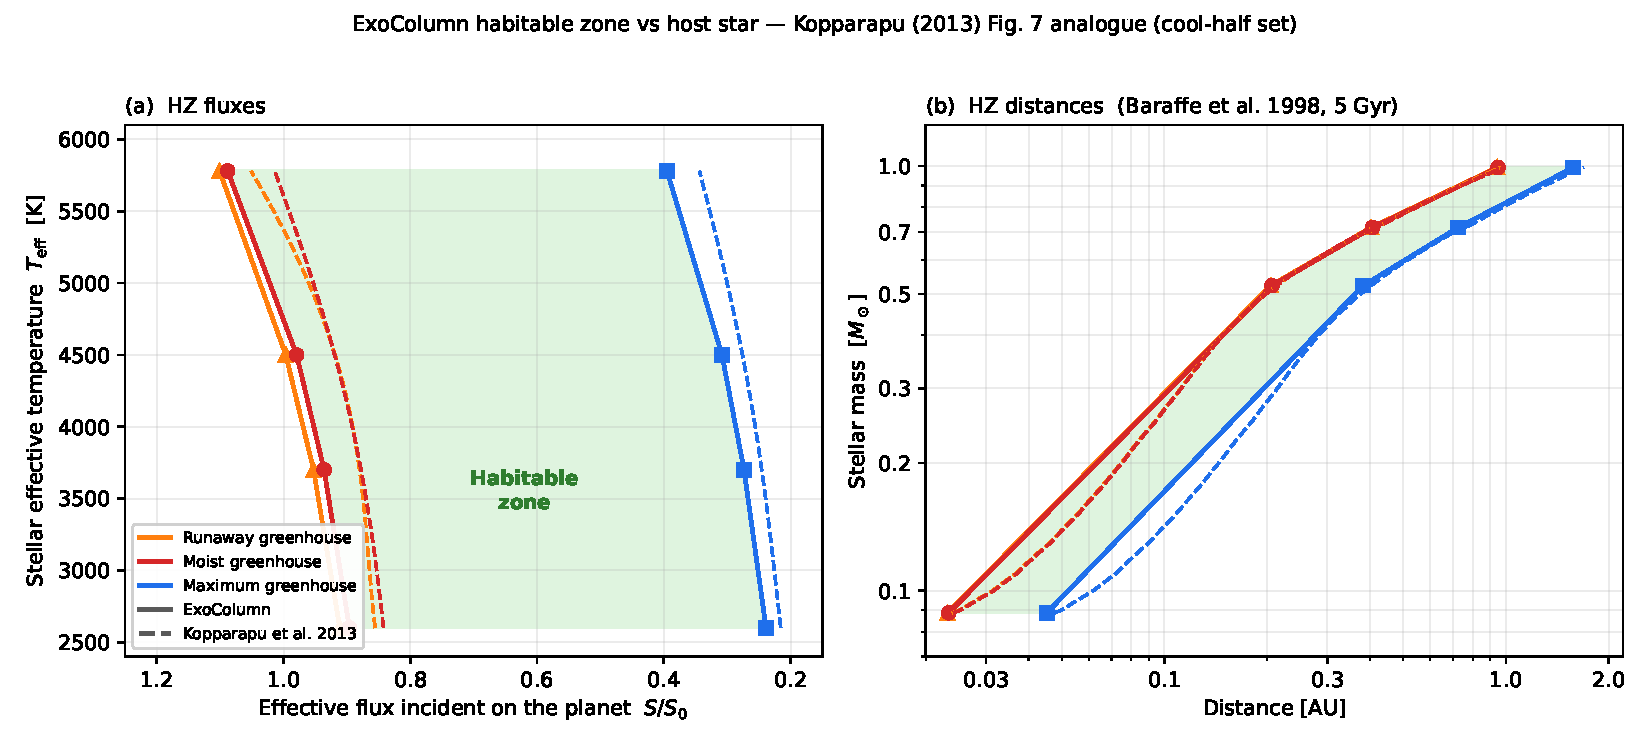
\includegraphics[width=0.65\textwidth]{reference/habitablezone/hz_figure7.pdf}
\caption{[HZ boundaries vs stellar effective temperature (analogue of Kopparapu
et al. 2013, Fig. 7). Top: $S_{\rm eff}$ at the moist- and maximum-greenhouse
limits vs $T_{\rm eff}$. Bottom: corresponding orbital distance vs stellar mass
from $d=\sqrt{(L/L_\odot)/S_{\rm eff}}$, using the Baraffe et al. (1998) 5 Gyr
solar-metallicity isochrone (the F star anchored to the present-day main
sequence). Solar System and TRAPPIST-1 planets shown for reference. Dashed =
Kopparapu (2013).]}
\label{fig:hz_fig7}
\end{figure}

%% The HZ boundary coefficients (the reusable deliverable) are auto-generated by
%% reference/habitablezone/hz_polyfit.py; its bracketed caption/comments are
%% regenerated on each run, so rewrite them in the script (not the .tex) or here.
% Auto-generated by reference/habitablezone/hz_polyfit.py -- do not edit by hand.
\begin{deluxetable*}{lrrrrr}
\tablecaption{}
\tablehead{
  \colhead{HZ boundary} & \colhead{$S_{\rm eff,\odot}$} &
  \colhead{$a$} & \colhead{$b$} & \colhead{$c$} & \colhead{$d$}
}
\startdata
Runaway greenhouse & 1.1015 & $9.4144\times10^{-5}$ & $7.3652\times10^{-9}$ & $-2.5772\times10^{-12}$ & $-4.6037\times10^{-16}$ \\
Moist greenhouse & 1.0880 & $9.5624\times10^{-5}$ & $5.4507\times10^{-9}$ & $-3.7032\times10^{-12}$ & $-5.9351\times10^{-16}$ \\
Maximum greenhouse & 0.3947 & $7.5232\times10^{-5}$ & $3.4318\times10^{-9}$ & $-3.3521\times10^{-12}$ & $-5.6844\times10^{-16}$
\enddata
\tablecomments{$S_{\rm eff}(T_{\rm eff}) = S_{\rm eff,\odot} + a\,T_\star + b\,T_\star^2 + c\,T_\star^3 + d\,T_\star^4$, with $T_\star = T_{\rm eff} - 5780$~K, valid for $T_{\rm eff} = 2000-7200$~K.}
\label{tab:hz_coeff}
\end{deluxetable*}


\section{Dependence on planetary mass} \label{sec:mass}
%% TODO
[HZ vs $T_{\rm eff}$ for 0.1, 1, and 5 $M_\oplus$. Mass sets surface gravity
($g=g_\oplus M^{0.375}\Rightarrow$ 4.14, 9.81, 17.93 m s$^{-2}$) and N$_2$
inventory ($p_{\rm N_2}=1\,{\rm bar}\,M^{0.75}\Rightarrow$ 0.18, 1.0, 3.34 bar);
gravity is set at compile time. Inner (runaway) $S_{\rm eff}$ at the Sun:
1.041 / 1.102 / 1.161 for 0.1 / 1 / 5 $M_\oplus$, vs Kopparapu (2014)
0.990 / 1.107 / 1.188 --- the 1 $M_\oplus$ case matches and the mass ordering
(higher gravity $\to$ thinner column $\to$ HZ farther in) is reproduced, with a
somewhat compressed spread.]

\begin{figure}[ht!]
\centering
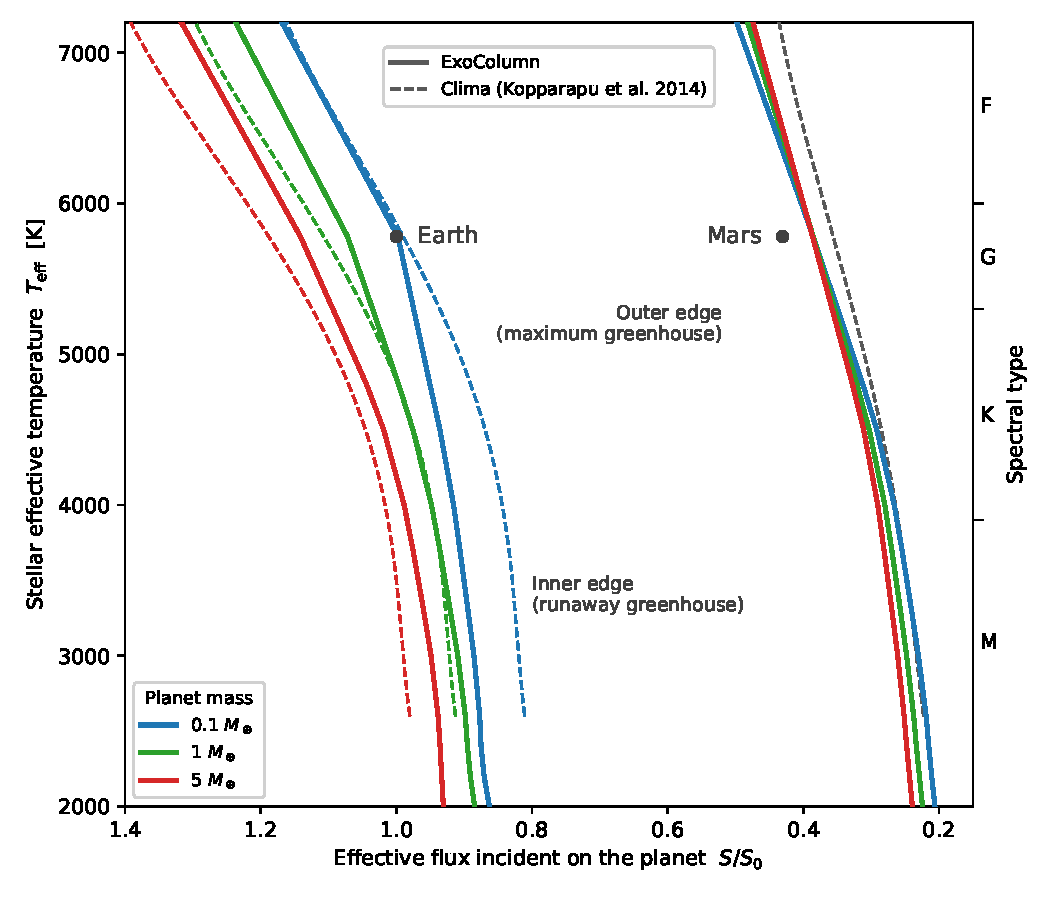
\includegraphics[width=0.7\textwidth]{reference/planet_mass/hz_mass.pdf}
\caption{[HZ dependence on planet mass (analogue of Kopparapu et al. 2014,
Fig. 3): HZ limits vs stellar effective temperature for 0.1, 1, and 5 $M_\oplus$
planets, which differ in surface gravity (4.14/9.81/17.93 m s$^{-2}$) and N$_2$
inventory (0.18/1.0/3.34 bar). Inner-edge (runaway) $S_{\rm eff}$ at the Sun is
1.041/1.102/1.161. Dashed = Kopparapu (2014) Eq. 4 (note: the 2014 runaway fit
lies $\sim$5--6\% above the 2013 fit used in Fig.~\ref{fig:hz_fig7}).]}
\label{fig:hz_mass}
\end{figure}

\section{Discussion} \label{sec:discussion}
%% TODO
[Limitations and offsets, quantified. (1) Cloud-free 1-D column. (2) The inner-HZ
$S_{\rm eff}$ runs $\approx$1.08--1.09 vs Kopparapu's 1.02--1.06; the LBL
benchmarks (Section~\ref{sec:lbl}) show both radiation cores are LBL-grade, so
this is the CLIMA-2013 ingredients (BPS near-IR continuum, $k$-distribution),
not a core error --- it is near-IR shortwave H$_2$O absorption (albedo 0.211 vs
0.193). (3) Surface-coupling resolution sensitivity $\sim$2 K in $T_s$.
(4) Cold-point warm bias $\approx204$ vs $\approx197$ K (ExoRT n68equiv vs
RRTMG). (5) Dense-CO$_2$ ($>$10 bar) $k$-table pressure extrapolation clamped.
Net effect: ExoColumn's HZ is conservative --- inner edge slightly farther in,
outer edge slightly closer in, than Kopparapu's.]

\section{Summary and conclusions} \label{sec:summary}
%% TODO
[ExoColumn is a fast 1-D RCE model with ExoCAM-consistent (ExoRT) radiation,
validated against modern Earth ($T_s=287.84$ K), LBL benchmarks (LBL-grade in
both LW and SW), and the Kopparapu HZ limits across F--M stars and 0.1--5
$M_\oplus$. We provide updated, ready-to-use HZ boundary coefficients
(Table~\ref{tab:hz_coeff}).]

%% ============================================================
%% Back matter
%% ============================================================

\begin{acknowledgments}
%% TODO
\end{acknowledgments}

%\facilities{}
%\software{}

%\appendix
%\section{} \label{sec:appendix}

\bibliography{ms}
\bibliographystyle{aasjournal}

\end{document}
